% vim: set textwidth=78 autoindent:

\subsection{Getrennter Text Plugin}\label{label_dltext}    

% when the revision of a section has been finalized, 
% comment out the following line:
%\updatedisclaimer

Mit dem Getrennter Text Plugin k�nnen ASCII-Texttabellen, die u.a zwei
Spalten f�r X- und Y-Koordinaten enthalten, als ein Layer in QGIS geladen werden.

\minisec{Anforderungen}

Um Datenspalten aus einer Textdatei in QGIS zu laden, muss diese Textdatei
bestimmte Eigenschaften aufweisen:

\begin{enumerate}
\item Eine Kopfzeile mit den Spaltennamen. Diese Kopfzeile muss die erste
Zeile der Datei sein
\item Die Textdatei muss mindestens eine Spalte mit X- und eine mit
Y-Koordinaten enthalten.
Die Bezeichnungen in der Kopfzeile f�r diese Spalten k�nnen beliebig sein.
\item Die X- und Y-Koordinaten m�ssen als Zahlen angegeben sein. Das
Koordinatensystem spielt keine Rolle.
\end{enumerate}

Als Beispiel f�r einen Textdatei importieren wir die Datei
\filename{elevp.csv} aus dem QGIS Beispieldatensatz \ref{label_sampledata}:

\begin{verbatim} 
X;Y;ELEV
-300120;7689960;13
-654360;7562040;52
1640;7512840;3
[...]
\end{verbatim}

Einige weitere Anmerkungen zu Textdateien:

\begin{enumerate}
\item  Die Beispieldatei verwendet \mbox{$|$} als Trennzeichen. Es k�nnen
auch andere Zeichen zum Trennen der Spalten verwendet werden.
\item Die erste Zeile ist die Kopfzeile. Sie enth�lt die Spaltennamen name,
latdec, longdec und cell
\item Anf�hrungszeichen ({\tt{}"{}}) d�rfen nicht als Trennzeichen benutzt
werden
\item Die X-Koordinaten sind in der Spalte {\em longdec} enthalten
\item Die Y-Koordinaten sind in der Spalte {\em latdec} enthalten
\end{enumerate}

\minisec{Das Plugin verwenden}

Um das Plugin zu benutzen, m�ssen Sie QGIS starten und den Plugin Manager
aufrufen, um das Plugin zu aktivieren:

Starten Sie QGIS, �ffnen Sie den Plugin Manager �ber das Men�
\mainmenuopt{Plugins} > \dropmenuopttwo{mActionShowPluginManager}{Plugins
verwalten}.\index{plugins!manager} Der Plugin Manager zeigt eine Liste
vorhandener Plugins. Sie k�nnen das  Plugins mit den entsprechenden
Kontrollk�stchen \checkbox{Getrennter Text} aktivieren und dann auf den Knopf 
\button{OK} klicken, wie in Kapitel \ref{sec:managing_plugins} beschrieben.

Klicken Sie nun auf das Icon \toolbtntwo{delimited_text}{Getrennter Text} in
der Werkzeugleiste, um den Dialog zu �ffnen (siehe
Abbildung~\ref{fig:delim_text_plugin_dialog}).

\begin{figure}[ht]
   \begin{center}
   \caption{Plugin Getrennter Text \nixcaption}\label{fig:delim_text_plugin_dialog}\smallskip
   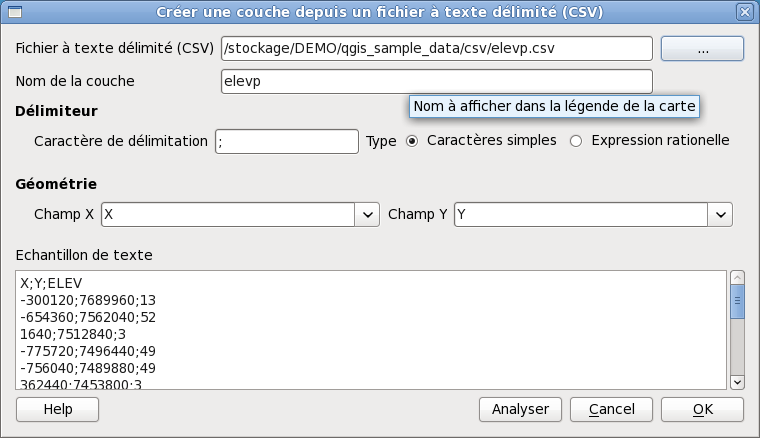
\includegraphics[clip=true, width=11cm]{delimited_text_dialog}
   \end{center}  
\end{figure}

Zuerst m�ssen Sie ein Trennzeichen f�r die Textspalten angeben. In diesem
Beispiel ist es das Trennzeichen \mbox{$;$}. Danach w�hlen Sie mit den Knopf
\button{Suchen} die Datei \filename{qgis\_sample\_data/csv/elevp.csv} aus. 

Damit die Textdatei richtig durchsucht werden kann, ist es wichtig, das
richtige Trennzeichen zu w�hlen. Im unteren Feld wird nun der Inhalt korrekt
in die vorkommenden Spalten unterteilt dargestellt.

W�hlen Sie nun die Spalten f�r die X- und Y-Koordinaten aus und tragen einen
Namen ein, unter dem die Daten in QGIS angezeigt werden sollen. Um die Daten
zu sehen, klicken Sie auf \button{Hinzuf�gen}. Der Layer verh�lt sich nun wie
jeder andere Vektorlayer in QGIS.

